% Created 2019-07-01 Mon 23:40
% Intended LaTeX compiler: pdflatex
\documentclass[11pt]{article}
\usepackage[utf8]{inputenc}
\usepackage[T1]{fontenc}
\usepackage{graphicx}
\usepackage{grffile}
\usepackage{longtable}
\usepackage{wrapfig}
\usepackage{rotating}
\usepackage[normalem]{ulem}
\usepackage{amsmath}
\usepackage{textcomp}
\usepackage{amssymb}
\usepackage{capt-of}
\usepackage{hyperref}
\usepackage{minted}
\author{Nicolás Luarte}
\date{\today}
\title{Javiera}
\hypersetup{
 pdfauthor={Nicolás Luarte},
 pdftitle={Javiera},
 pdfkeywords={},
 pdfsubject={},
 pdfcreator={Emacs 25.2.2 (Org mode 9.2.3)}, 
 pdflang={English}}
\begin{document}

\maketitle
\tableofcontents

\section{Ciclos}
\label{sec:orga086c8f}
\begin{center}
\begin{tabular}{lll}
Ejercicio & Protocolo & Bloque\\
\hline
Sentadilla de competencia & x6@8, 10\%, 4x6 & A\\
Sentadilla con pausa (3 ct) & x6@8, 10\%, 2x6 & A\\
Banca de competencia & x6@8, 10\%, 4x7 & A\\
Banca agarre cerrado & x6@8, 10\%, 2x7 & A\\
\hline
Press banca triple pausa & x6@8, 10\%, 3x7 & B\\
Peso muerto de competencia & x3@8, 15\%, 3x4 & B\\
Peso muerto con pausa (3 ct) & x3@8, 15\%, 2x4 & B\\
Peso muerto desde bloques & x3@8, 15\%, 2x5 & B\\
\end{tabular}
\end{center}

\section{Comentarios técnicos}
\label{sec:orgd881742}
\section{Registro de progreso}
\label{sec:org3f0703d}
\begin{center}
\label{tab:org7397e3d}
\begin{tabular}{llll}
Ejercicio & RPE & Peso & Fecha\\
\hline
 &  &  & \\
\end{tabular}
\end{center}
\begin{center}
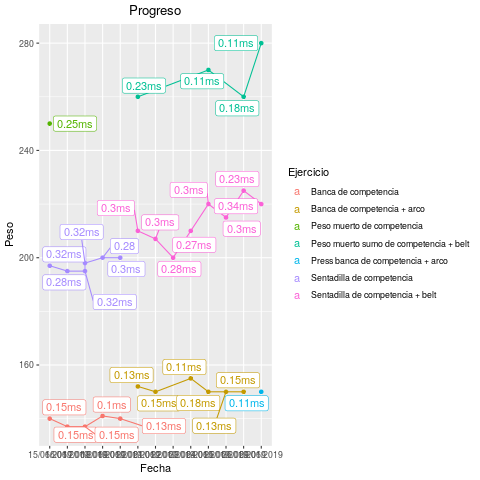
\includegraphics[width=.9\linewidth]{tmp.png}
\end{center}
\end{document}
